\documentclass{beamer}\usepackage[]{graphicx}\usepackage[]{color}
% maxwidth is the original width if it is less than linewidth
% otherwise use linewidth (to make sure the graphics do not exceed the margin)
\makeatletter
\def\maxwidth{ %
  \ifdim\Gin@nat@width>\linewidth
    \linewidth
  \else
    \Gin@nat@width
  \fi
}
\makeatother

\definecolor{fgcolor}{rgb}{0.345, 0.345, 0.345}
\newcommand{\hlnum}[1]{\textcolor[rgb]{0.686,0.059,0.569}{#1}}%
\newcommand{\hlstr}[1]{\textcolor[rgb]{0.192,0.494,0.8}{#1}}%
\newcommand{\hlcom}[1]{\textcolor[rgb]{0.678,0.584,0.686}{\textit{#1}}}%
\newcommand{\hlopt}[1]{\textcolor[rgb]{0,0,0}{#1}}%
\newcommand{\hlstd}[1]{\textcolor[rgb]{0.345,0.345,0.345}{#1}}%
\newcommand{\hlkwa}[1]{\textcolor[rgb]{0.161,0.373,0.58}{\textbf{#1}}}%
\newcommand{\hlkwb}[1]{\textcolor[rgb]{0.69,0.353,0.396}{#1}}%
\newcommand{\hlkwc}[1]{\textcolor[rgb]{0.333,0.667,0.333}{#1}}%
\newcommand{\hlkwd}[1]{\textcolor[rgb]{0.737,0.353,0.396}{\textbf{#1}}}%
\let\hlipl\hlkwb

\usepackage{framed}
\makeatletter
\newenvironment{kframe}{%
 \def\at@end@of@kframe{}%
 \ifinner\ifhmode%
  \def\at@end@of@kframe{\end{minipage}}%
  \begin{minipage}{\columnwidth}%
 \fi\fi%
 \def\FrameCommand##1{\hskip\@totalleftmargin \hskip-\fboxsep
 \colorbox{shadecolor}{##1}\hskip-\fboxsep
     % There is no \\@totalrightmargin, so:
     \hskip-\linewidth \hskip-\@totalleftmargin \hskip\columnwidth}%
 \MakeFramed {\advance\hsize-\width
   \@totalleftmargin\z@ \linewidth\hsize
   \@setminipage}}%
 {\par\unskip\endMakeFramed%
 \at@end@of@kframe}
\makeatother

\definecolor{shadecolor}{rgb}{.97, .97, .97}
\definecolor{messagecolor}{rgb}{0, 0, 0}
\definecolor{warningcolor}{rgb}{1, 0, 1}
\definecolor{errorcolor}{rgb}{1, 0, 0}
\newenvironment{knitrout}{}{} % an empty environment to be redefined in TeX

\usepackage{alltt}
%\documentclass[handout]{beamer}
\mode<presentation>
{
  \usetheme{Madrid}      % or try Darmstadt, Madrid, Warsaw, ...
  \usecolortheme{default} % or try albatross, beaver, crane, ...
  \usefonttheme{default}  % or try serif, structurebold, ...
  \setbeamertemplate{navigation symbols}{}
  \setbeamertemplate{caption}[numbered]
} 
\definecolor{darkblue}{rgb}{0.01,0.24,0.40}

%\usepackage[table]{xcolor}

\let\tnote\relax  % threeparttable defines \tnore

\usepackage{adjustbox}
\usepackage{amsmath,mathtools}
\usepackage{array}
\usepackage[english]{babel}
\usepackage{blindtext}
\usepackage{booktabs}
\usepackage{colortbl,xcolor}
\usepackage{float}
\usepackage[T1]{fontenc}    % citation
\usepackage[bottom]{footmisc}
\usepackage{graphicx}
\usepackage{grffile}  % to check for known picture extensions
\usepackage{hyperref}
\usepackage[utf8]{inputenc}  % citation 
\usepackage{lmodern}
\usepackage{longtable}
\usepackage{makecell}
\usepackage{multirow}
\usepackage{multicol}
\usepackage{natbib}
\usepackage[super]{nth}
\usepackage{pdflscape}
\usepackage{tabu}
\usepackage{threeparttable,threeparttablex}
\usepackage[normalem]{ulem}
\usepackage[absolute, overlay]{textpos}
\usepackage{pgfplots}
%\usepackage{ctable} % has to be after tikz
\usepackage{wrapfig}
\usepackage{fancyhdr}
\usepackage{fancybox}    % \Ovalbox \ovalbox \doublebox \shadowbox
\usepackage{setspace}
\let\counterwithout\relax
\let\counterwithin\relax
\usepackage{chngcntr}

\pgfplotsset{compat=1.16}
\usepackage{tikz}
\usetikzlibrary{shapes}  % bubble graphs
\usetikzlibrary{arrows}
\usetikzlibrary{positioning}
\usetikzlibrary{calc}

% For Beamer to functionate 
\usepackage{beamer}
\usepackage{atbegshi}
\usepackage{etoolbox}
\usepackage{hyperref}
\usepackage{ifpdf}
\usepackage{pgf}
\usepackage{translator}
%\usepackage{Sweave}



\newcommand\blfootnote[1]{% command to make "blind-foot-note"
\begingroup
\renewcommand\thefootnote{}\footnote{#1}%
\addtocounter{footnote}{-1}%
\endgroup
}


\AtBeginSection[]{
  \begin{frame}
  \vfill
  \centering
  \begin{beamercolorbox}[sep=8pt,center,shadow=true,rounded=true]{title}
    \usebeamerfont{title}\insertsectionhead\par%
  \end{beamercolorbox}
  \vfill
  \end{frame}
}


\definecolor{darkblue}{rgb}{0.01,0.24,0.40}
\usecolortheme[named=darkblue]{structure}

\setbeamercolor{section in head/foot}{fg=white, bg=darkblue}

%\renewcommand*{\blfootnote}{\scriptsize} 

\makeatletter

\setbeamertemplate{footline}
{
  \leavevmode
  \hbox{ 
  \begin{beamercolorbox}[wd=.333333\paperwidth,ht=2.25ex,dp=1ex,center]{section in head/foot}%
    \usebeamerfont{author in head/foot} \insertshorttitle
  \end{beamercolorbox}%
  \begin{beamercolorbox}[wd=.333333\paperwidth,ht=2.25ex,dp=1ex,center]{section in head/foot}%
    \usebeamerfont{title in head/foot}\insertsection
  \end{beamercolorbox}%
  \begin{beamercolorbox}[wd=.333333\paperwidth,ht=2.25ex,dp=1ex,right]{section in head/foot}%
    \usebeamerfont{date in head/foot}\insertshortdate{}\hspace*{2em}
    \insertframenumber{} / \inserttotalframenumber\hspace*{2ex} 
  \end{beamercolorbox} }%
  \vskip0pt%
}
\setbeamertemplate{blocks}[default]
%\addtobeamertemplate{footnote}{}{\vspace{2ex}}

\makeatother

\title[Sebastián Riera, Ph.D.]{Análisis de la experiencia del Fondo Potrerillos y su posible extensión a otras áreas bajo riego de Mendoza.\\ Aspectos económicos-financieros, jurídicos, ambientales y de desarrollo territorial} 

\author{M.Sc. Lic. Sebastian Riera, Ph.D.}
\institute{Avances en materia económica - 2019}   % 
\date{11.02.2020}
\IfFileExists{upquote.sty}{\usepackage{upquote}}{}
\begin{document}
%\SweaveOpts{concordance=TRUE}
{
\setbeamertemplate{footline}{}   
\begin{frame} \vspace*{.5cm}\titlepage  
  %\vspace*{-1cm} \small
  \begin{columns}
    \column{.4\linewidth}
    \includegraphics[width = .6\textwidth]{/Users/SebastianRiera/Documents/TesisCloud/figures/{LogoFcaVerde}.png}
       \column{.4\linewidth}
    \includegraphics[width = .5\textwidth]{/Users/SebastianRiera/Documents/TesisCloud/figures/{LogoUncuyo}.png}
    \column{.5\linewidth}
    \includegraphics[width = .5\textwidth]{/Users/SebastianRiera/Downloads/{LogoDgi}.png}
  \end{columns}
\end{frame}
}
\addtocounter{framenumber}{-1}















\begin{knitrout}
\definecolor{shadecolor}{rgb}{0.969, 0.969, 0.969}\color{fgcolor}\begin{kframe}


{\ttfamily\noindent\bfseries\color{errorcolor}{\#\# Error in aggregate(Dgi2020\$metros, by = list(Dgi2020\$Subdelegacion), FUN = sum, : object 'Dgi2020' not found}}

{\ttfamily\noindent\bfseries\color{errorcolor}{\#\# Error in number(x, accuracy = accuracy, scale = scale, prefix = prefix, : object 'Rev2020' not found}}

{\ttfamily\noindent\bfseries\color{errorcolor}{\#\# Error in rownames(Revestimiento) <- c("{}Atuel"{}, "{}Diamante"{}, "{}Malargüe"{}, : object 'Revestimiento' not found}}\end{kframe}
\end{knitrout}

\begin{knitrout}
\definecolor{shadecolor}{rgb}{0.969, 0.969, 0.969}\color{fgcolor}\begin{kframe}


{\ttfamily\noindent\bfseries\color{errorcolor}{\#\# Error in rbind(Mza17, Mza18, Mza19, Mza20, fill = TRUE): object 'Mza20' not found}}

{\ttfamily\noindent\bfseries\color{errorcolor}{\#\# Error in merge(x = Mendoza, y = EfMendoza[, c(2:4, 6, 13, 15, 17:21, 24:28, : object 'Mendoza' not found}}

{\ttfamily\noindent\bfseries\color{errorcolor}{\#\# Error in merge(x = Mendoza, y = CaudalWebQ, by = c("{}CodigoCauce"{}), all.x = TRUE): object 'Mendoza' not found}}

{\ttfamily\noindent\itshape\color{messagecolor}{\#\# Linking to GEOS 3.7.2, GDAL 2.4.2, PROJ 5.2.0}}

{\ttfamily\noindent\bfseries\color{errorcolor}{\#\# Error in merge(x = Mendoza, y = umendoza[, c(2, 4)], by = c("{}Inspeccion"{}), : object 'Mendoza' not found}}

{\ttfamily\noindent\bfseries\color{errorcolor}{\#\# Error in eval(lhs, parent, parent): object 'Mendoza' not found}}

{\ttfamily\noindent\bfseries\color{errorcolor}{\#\# Error in arrange(Mendoza, CodigoCauce): object 'Mendoza' not found}}

{\ttfamily\noindent\bfseries\color{errorcolor}{\#\# Error in eval(expr, envir, enclos): object 'Mendoza' not found}}

{\ttfamily\noindent\bfseries\color{errorcolor}{\#\# Error in eval(expr, envir, enclos): object 'Mendoza' not found}}

{\ttfamily\noindent\bfseries\color{errorcolor}{\#\# Error in eval(expr, envir, enclos): object 'Mendoza' not found}}

{\ttfamily\noindent\bfseries\color{errorcolor}{\#\# Error in eval(expr, envir, enclos): object 'Mendoza' not found}}

{\ttfamily\noindent\bfseries\color{errorcolor}{\#\# Error in eval(expr, envir, enclos): object 'Mendoza' not found}}

{\ttfamily\noindent\bfseries\color{errorcolor}{\#\# Error in eval(expr, envir, enclos): object 'Mendoza' not found}}

{\ttfamily\noindent\bfseries\color{errorcolor}{\#\# Error in ifelse(Mendoza\$inversion == 845000, (Mendoza\$Q0) * (Mendoza\$EfPost - : object 'Mendoza' not found}}

{\ttfamily\noindent\bfseries\color{errorcolor}{\#\# Error in eval(expr, envir, enclos): object 'Mendoza' not found}}

{\ttfamily\noindent\bfseries\color{errorcolor}{\#\# Error in eval(expr, envir, enclos): object 'Mendoza' not found}}

{\ttfamily\noindent\bfseries\color{errorcolor}{\#\# Error in eval(expr, envir, enclos): object 'Mendoza' not found}}

{\ttfamily\noindent\bfseries\color{errorcolor}{\#\# Error in eval(expr, envir, enclos): object 'Mendoza' not found}}

{\ttfamily\noindent\bfseries\color{errorcolor}{\#\# Error in eval(expr, envir, enclos): object 'Mendoza' not found}}

{\ttfamily\noindent\bfseries\color{errorcolor}{\#\# Error in eval(expr, envir, enclos): object 'Mendoza' not found}}

{\ttfamily\noindent\bfseries\color{errorcolor}{\#\# Error in eval(expr, envir, enclos): object 'Mendoza' not found}}

{\ttfamily\noindent\bfseries\color{errorcolor}{\#\# Error in eval(expr, envir, enclos): object 'Mendoza' not found}}

{\ttfamily\noindent\bfseries\color{errorcolor}{\#\# Error in is.data.frame(x): object 'Mendoza' not found}}

{\ttfamily\noindent\bfseries\color{errorcolor}{\#\# Error in as.data.frame(Mendoza[, c(10, 13, 9, 5, 7, 33, 32, 34:36, 42:44)]): object 'Mendoza' not found}}

{\ttfamily\noindent\bfseries\color{errorcolor}{\#\# Error in as.data.frame(Mendoza[c(1:7, 9:27), c(9, 12, 8, 26, 4:5, 31, : object 'Mendoza' not found}}

{\ttfamily\noindent\bfseries\color{errorcolor}{\#\# Error in eval(lhs, parent, parent): object 'Mendoza' not found}}\end{kframe}
\end{knitrout}

\begin{knitrout}
\definecolor{shadecolor}{rgb}{0.969, 0.969, 0.969}\color{fgcolor}\begin{kframe}


{\ttfamily\noindent\bfseries\color{errorcolor}{\#\# Error in eval(expr, envir, enclos): object 'Mendoza' not found}}

{\ttfamily\noindent\bfseries\color{errorcolor}{\#\# Error in eval(expr, envir, enclos): object 'OfertaMza' not found}}

{\ttfamily\noindent\bfseries\color{errorcolor}{\#\# Error in eval(expr, envir, enclos): object 'Mendoza' not found}}

{\ttfamily\noindent\bfseries\color{errorcolor}{\#\# Error in eval(expr, envir, enclos): object 'OfertaMza1' not found}}

{\ttfamily\noindent\bfseries\color{errorcolor}{\#\# Error in eval(expr, envir, enclos): object 'Mendoza' not found}}

{\ttfamily\noindent\bfseries\color{errorcolor}{\#\# Error in eval(expr, envir, enclos): object 'OfertaMza2' not found}}

{\ttfamily\noindent\bfseries\color{errorcolor}{\#\# Error in mean(OfertaMza\$valueEfBis, na.rm = T): object 'OfertaMza' not found}}

{\ttfamily\noindent\bfseries\color{errorcolor}{\#\# Error in mean(OfertaMza2\$valueAhorro, na.rm = T): object 'OfertaMza2' not found}}

{\ttfamily\noindent\bfseries\color{errorcolor}{\#\# Error in eval(expr, envir, enclos): object 'OfertaMza1' not found}}

{\ttfamily\noindent\bfseries\color{errorcolor}{\#\# Error in eval(expr, envir, enclos): object 'AhorroCtoPromedio' not found}}

{\ttfamily\noindent\bfseries\color{errorcolor}{\#\# Error in ggplot(OfertaMza): object 'OfertaMza' not found}}

{\ttfamily\noindent\bfseries\color{errorcolor}{\#\# Error in ggplot(OfertaMza1): object 'OfertaMza1' not found}}

{\ttfamily\noindent\bfseries\color{errorcolor}{\#\# Error in ggplot(OfertaMza2): object 'OfertaMza2' not found}}\end{kframe}
\end{knitrout}


\begin{frame}{Resumen}
 \footnotesize \tableofcontents
\end{frame}

% Body document 

\section[Introducción]{Introducción}

% Intro Context
\subsection{Motivación}

\begin{frame}{Motivación}
 \begin{itemize}
       \item Dificultades de manejo del recurso hídrico en contexto de escasez 
\pause \item Análisis profundo $\rightarrow$ sistema resiliente a fenómenos del CC
\pause \item Ámbitos económicos y jurídicos del Fondo Potrerillos y posibles extensiones \\
\pause \item Desafío es adaptar instrumentos económicos al manejo de activos complejos como el agua
% \pause \item Análisis económico permite el diseño de herramientas eficientes para mejorar la gobernanza del agua en contexto de conflicto de intereses y altos costos de transacción
\pause \item Conflicto de intereses y altos costos de transacción $\rightarrow$ diseño de herramientas eficientes para mejorar la gobernanza del agua
    \end{itemize}
    \blfootnote{\scriptsize \citep{Gomez2018,MAGyP2011b,Scheierling2016,Gruere2019}} 
    
\end{frame}

\subsection{Objetivos}
\begin{frame}{Objetivos}

\textcolor{green}{\textbf{Generales}} \\

Considerar herramientas integrales desde el pdv económico y jurídico que contribuyan a solucionar la dotación de agua con demandas crecientes en períodos de escasez en climas semi-áridos

Aplicar elementos de política económica en la planificación manejo del recurso hídrico 

\pause \vspace{3pt}
\textcolor{darkblue}{\textbf{Específicos}}
\begin{itemize}
\item Estimación del costo de ahorro de agua por la inversión en infraestructura de riego por Subdelegación

\item Adaptar el rango de valores de costos acorde a las características productivas, usos del suelo y sistemas de riego asociados
\end{itemize}
      \blfootnote{\scriptsize \citep{Pittock2016}}
\end{frame}


\begin{frame}{Aspectos jurídicos}
\vspace{-2pt}

Revisión de antecedentes jurídicos que dan sustento a las resoluciones:
\begin{itemize}
\item R576/00 HTA
\item R34/01 HTA
\item R945/06 HTA
\item R299/07 HTA
\end{itemize}
\end{frame}


\begin{frame}{Aspectos económicos}
Modelo económico integral
\pause \vspace{2pt}
    \begin{itemize}
      \item Aproximación al costo de oportunidad (económico)
      \item Efectos de la tecnificación en riego en valores económicos
      \item Efectos de inversiones sobre la productividad de los cultivos 
      \item Estimación de productividad marginal del agua
    \end{itemize}

\end{frame}


\section{Modelo económico general}

\begin{frame}{Respecto a la eficiencia}
Conceptos generales

\begin{itemize}
          \item \textcolor{darkblue}{\textbf{Eficiencia de conducción ($EfC$)}}: redes de canales y conductos desde la desviación del río, el embalse o estación de bombeo hasta las tomas del sistema de distribución.
    \pause \item \textcolor{red}{\textbf{Eficiencia de distribución ($EfD$)}}: de los canales y conductos de distribución $\rightarrow$ red de transporte a campos individuales
    \pause \item \textcolor{green}{\textbf{Eficiencia de aplicación ($EfA$)}}: relación entre dotación de agua entregada y la cantidad de agua necesaria y disponible
\end{itemize}

\pause
\begin{block}{Eficiencia sistema}
 $\textcolor{darkblue}{\textbf{EfC}} \times \textcolor{red}{\textbf{EfD}} \times \textcolor{green}{\textbf{EfA}}$
\end{block}
      \blfootnote{\scriptsize \citep{Bos1990,Morabito2005}}
\end{frame}

\begin{frame}{How blocks help in perfect phylogeny haplotyping.}
  \begin{enumerate}
  \item Partition the site set into overlapping contiguous blocks.
  \item Compute a perfect phylogeny for each block and combine them.
  \item Use dynamic programming for finding the partition.
  \end{enumerate}

  \begin{tikzpicture}
    \useasboundingbox (0,-1) rectangle (10,2);
    
    \draw[line width=2mm,dash pattern=on 1mm off 1mm]
      (0,1) -- (9.99,1) node[midway,above] {Genotype matrix}
      (0,0.6666) -- (9.99,0.6666)
      (0,0.3333) -- (9.99,0.3333)
      (0,0) -- (9.99,0) node[midway,below] {\only<1>{no perfect phylogeny}};

    \begin{scope}[xshift=-.5mm]
      \only<2->
      {
        \draw[red,block]            (0,.5)   -- (3,.5)
          node[midway,below] {perfect phylogeny};
      }
        
      \only<3->
      {
        \draw[green!50!black,block] (2.5,.5)   -- (7,.5)
          node[pos=0.6,below] {perfect phylogeny};
      }

      \only<4->
      {
        \draw[blue,block]           (6.5,.5) -- (10,.5)
          node[pos=0.6,below] {perfect phylogeny};
      }
    \end{scope}
  \end{tikzpicture}
\end{frame}


\begin{frame}{Estimación de la oferta hídrica adicional}
\vspace{-3pt}
\begin{equation*}
\mathbb{A}_i^O = g (\bar{\mathbb{A}}^O, N_i, I_i, m_i^3, OF_i)
\end{equation*} \vspace{-2pt}
\pause
\begin{equation}
\mathbb{A}_i^{O} = \sum_{j=1}^{n} \Delta metros \times Q_{m^{3}/año} \times \Delta pérdida
\end{equation} \vspace{-2pt}

\begin{equation*}
\Delta Pérdida = \frac{EfC_{1} - EfC_{0}}{distancia \: media}
\end{equation*}

\pause  \begin{columns}
    \column{.3\linewidth}
  \begin{footnotesize}
$\bar{\mathbb{A}}^O$ caudal promedio \\
$N_i$ volumen de nieve \\
$I_i$ inversiones revestimiento \\
$m_i^3$ metros cúbicos adicionales \\
$OF_i$ otros factores
\end{footnotesize}

\pause \column{.6\linewidth}
\begin{figure}[H] \begin{center} 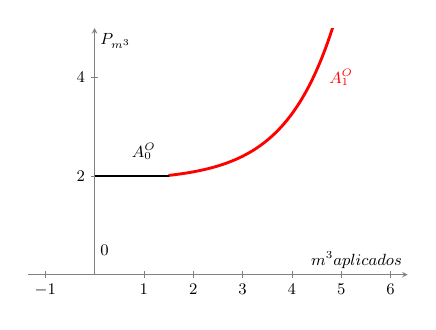
\begin{tikzpicture}[scale=.65]\small
\begin{axis}[axis line style=gray,
	samples=120,
	width=9.0cm,height=6.4cm,
	xmin=0, xmax=5,
	ymin=0, ymax=5,
	restrict y to domain=1:8,
	ytick={},
	xtick={},
	axis equal,
	axis x line=center,
	axis y line=center,
	xlabel=$m^{3} aplicados$,ylabel=$P_{m^{3}}$]
\addplot[red,domain=1.5:6,ultra thick]{exp(x-3)/2+1.9};
\addplot[ultra thick,black, domain=0:1.5]{2};
\addplot[] coordinates {(1,2.5)} node{$\mathbb{A}_0^O$};
\addplot[red] coordinates {(5,4)} node{$\mathbb{A}_1^O$};
\path (axis cs:0,0) node [anchor=north west,yshift=0.7cm] {0};
\end{axis} \end{tikzpicture} \\
\end{center}
\end{figure}

\end{columns}
\end{frame}




\section{Resultados preliminares}
\begin{frame}{Resultados preliminares}
\begin{knitrout}
\definecolor{shadecolor}{rgb}{0.969, 0.969, 0.969}\color{fgcolor}\begin{kframe}


{\ttfamily\noindent\bfseries\color{errorcolor}{\#\# Error in eval(lhs, parent, parent): object 'Revestimiento' not found}}\end{kframe}
\end{knitrout}
\end{frame}

%\begin{frame}{Resultados preliminares}
%<< DataObrasFull, results='hide', echo=FALSE, cache=FALSE>>=
%@

%<< SumFull, results='hide', echo=FALSE, cache=FALSE>>=
%@
%\end{frame}

\subsection{Subdelegación Río Mendoza}
\begin{frame}{Río Mendoza}

\begin{knitrout}
\definecolor{shadecolor}{rgb}{0.969, 0.969, 0.969}\color{fgcolor}\begin{kframe}


{\ttfamily\noindent\bfseries\color{errorcolor}{\#\# Error in as.data.frame(OfertaMza1[order(AAcum)]): object 'OfertaMza1' not found}}

{\ttfamily\noindent\bfseries\color{errorcolor}{\#\# Error in eval(expr, envir, enclos): object 'OfertaMzaInv' not found}}

{\ttfamily\noindent\bfseries\color{errorcolor}{\#\# Error in eval(lhs, parent, parent): object 'OfertaMzaInv' not found}}

{\ttfamily\noindent\bfseries\color{errorcolor}{\#\# Error in rbind(round(OfertaMzaInv\$InvAcum[[18]], digits = 0), round(OfertaMzaInv\$AAcum[[18]]/1000, : object 'OfertaMzaInv' not found}}

{\ttfamily\noindent\bfseries\color{errorcolor}{\#\# Error in rownames(MzaSum) = c("{}Inv. USD"{}, "{}Ahorro agua ('000 m3)"{}, "{}Caudal ahorrado (m3/s)"{}): object 'MzaSum' not found}}\end{kframe}
\end{knitrout}

\begin{kframe}


{\ttfamily\noindent\bfseries\color{errorcolor}{\#\# Error in eval(expr, envir, enclos): object 'MzaTable' not found}}\end{kframe}
\end{frame}

\begin{frame}{Río Mendoza}

\includegraphics[width=11.5cm,height=6.0cm]{/Users/SebastianRiera/Google Drive/Laboro/ResearchProposals/UNCuyo/UNCuyoIrrigacion/FcaIrrigacion/FcaIrrigacion/DgiData/Graphs/{OfertaMzaUm}.png}

\end{frame}

\begin{frame}{Resultados preliminares}
\begin{knitrout}
\definecolor{shadecolor}{rgb}{0.969, 0.969, 0.969}\color{fgcolor}\begin{kframe}


{\ttfamily\noindent\bfseries\color{errorcolor}{\#\# Error in as.data.frame(OfertaMza1[order(AAcum)]): object 'OfertaMza1' not found}}

{\ttfamily\noindent\bfseries\color{errorcolor}{\#\# Error in eval(expr, envir, enclos): object 'OfertaMzaInv' not found}}

{\ttfamily\noindent\bfseries\color{errorcolor}{\#\# Error in eval(lhs, parent, parent): object 'OfertaMzaInv' not found}}

{\ttfamily\noindent\bfseries\color{errorcolor}{\#\# Error in rbind(round(OfertaMzaInv\$InvAcum[[18]], digits = 0), round(OfertaMzaInv\$AAcum[[18]]/1000, : object 'OfertaMzaInv' not found}}

{\ttfamily\noindent\bfseries\color{errorcolor}{\#\# Error in rownames(MzaSum) = c("{}Inv. USD"{}, "{}Ahorro agua ('000 m3)"{}, "{}Caudal ahorrado (m3/s)"{}): object 'MzaSum' not found}}\end{kframe}
\end{knitrout}

\begin{knitrout}
\definecolor{shadecolor}{rgb}{0.969, 0.969, 0.969}\color{fgcolor}\begin{kframe}


{\ttfamily\noindent\bfseries\color{errorcolor}{\#\# Error in eval(lhs, parent, parent): object 'MzaSum' not found}}\end{kframe}
\end{knitrout}
\end{frame}








\subsection{Limitaciones $\&$ futuros pasos}
\begin{frame}{Limitaciones $\&$ futuros pasos}
  Limitaciones
  \begin{itemize}
         \item Información no sistematizada          
  \pause \item Metodología de análisis para \textcolor{red}{Eficiencia de distribución ($EfD$)}
  \pause \item Diferencias entre obras por administración y licitaciones
  \end{itemize}
  
  Futuros pasos
  \begin{itemize}
         \item Revisar enfoques que incorporen análisis de la distribución          
  \pause \item Estimar demandas actuales y potenciales efectos
  \pause \item Análisis extensivo al resto de las cuencas
  \end{itemize}
\end{frame}

\begin{frame}{Futuros pasos}
 \begin{figure} \begin{center} 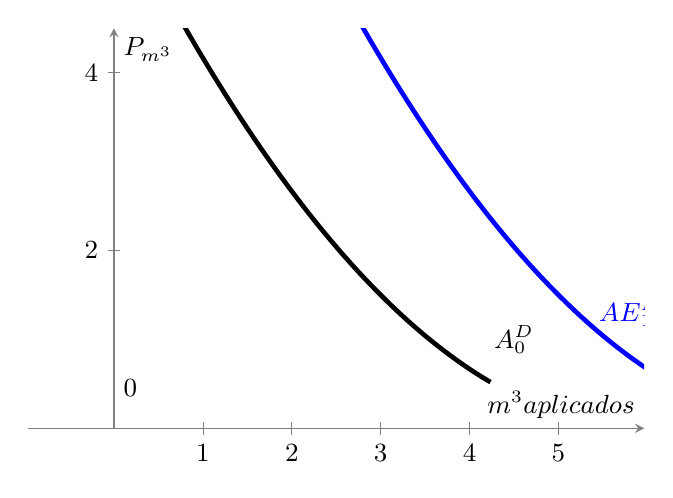
\begin{tikzpicture}[scale=1.0544]\small
\begin{axis}[axis line style=gray,
	samples=120,
	width=9.0cm,height=6.4cm,
	xmin=0, xmax=5,
	ymin=0, ymax=4.5,
	restrict y to domain=.5:5.5,
	ytick={},
	xtick={},
	axis equal,
	axis x line=center,
	axis y line=center,
	xlabel=$ m^{3} \space aplicados$, ylabel= $P_{m^{3}}$ ]
\addplot[ultra thick, blue,domain=0:6]{(x-8)^2/6};
\addplot[ultra thick,black, domain=0:6]{(x-6)^2/6};
\addplot[] coordinates {(4.5,1)} node{$\mathbb{A}_0^D$};
\addplot[blue] coordinates {(5.8,1.3)} node{$\mathbb{AE}_1^D$};
\path (axis cs:0,0) node [anchor=north west,yshift=0.7cm] {0};
\end{axis} \end{tikzpicture} \\
\caption{\label{DemandaAgua}Representación de la demanda de agua y agua efectiva $\mathbb{A}_0^D \ y \ \mathbb{AE}_1^D$}
\end{center}
\end{figure}

\end{frame}

\begin{frame}{Modelo económico integral}

\begin{figure}[h]
\begin{center} \begin{tikzpicture}[scale=.544]\small
\begin{axis}[axis line style=gray,
	samples=120,
	width=18.0cm,height=12.8cm,
	xmin=-5, xmax=5,
	ymin=-4.5, ymax=4.5,
	restrict y to domain=-5.5:5.5,
	ytick={},
	xtick={},
	axis equal,
	axis x line=center,
	axis y line=center,
	xlabel=$m^{3} \space aplicados$, ylabel= $P_{m^{3}}$]
\addplot[ultra thick,blue,domain=0:6]{(x-8)^2/6};
\addplot[ thick,black, domain=0:6]{(x-6)^2/6};
\addplot[] coordinates {(5,.5)} node{$\mathbb{A}_0^D$};
\addplot[blue] coordinates {(6,1.3)} node{$\mathbb{AE}_1^D$};
\addplot[ultra thick,red,domain=1.5:6]{exp(x-3)/2+1.9};
\addplot[ thick,black, domain=0:1.5]{2};
\addplot[] coordinates {(1,2.2)} node{$\mathbb{A}_0^O$};
\addplot[red] coordinates {(5,4)} node{$\mathbb{A}_1^O$};
\addplot[brown, thick, domain=-5:5]{-x};
\addplot[ultra thick, teal, domain=-5:0]{-1/35*(x+6)^(3)-0.5};
\addplot[teal] coordinates {(-6,-.7)} node{$PMg_i^{AE}$};
\addplot[black] coordinates {(-6,.4)} node{$CMg_{Agua}$};
\addplot[black] coordinates {(1,-4)} node{$Hm^3 \ efectivos$};
\addplot[brown] coordinates {(5.3,-4)} node{$tecnología \ riego$};
\path (axis cs:0,0) node [anchor=north west,yshift=0.7cm] {0};
\end{axis} \end{tikzpicture} \\
\caption{\label{Modelo}Representación de cambios en la demanda de agua $\mathbb{A}_i^D$ acorde a la expansión de la oferta de riego $\mathbb{A}_1^S$}
\end{center}
\end{figure}

\end{frame}

\begin{frame}{Modelo económico integral}

\begin{figure}[h]
\begin{center} \begin{tikzpicture}[scale=.544]\small
\begin{axis}[axis line style=gray,
	samples=120,
	width=18.0cm,height=12.8cm,
	xmin=-5, xmax=5,
	ymin=-4.5, ymax=4.5,
	restrict y to domain=-5.5:5.5,
	ytick={},
	xtick={},
	axis equal,
	axis x line=center,
	axis y line=center,
	xlabel=$m^{3} \space aplicados$, ylabel= $P_{m^{3}}$]
\addplot[ultra thick,blue,domain=0:6]{(x-8)^2/6};
\addplot[ thick,black, domain=0:6]{(x-6)^2/6};
\addplot[] coordinates {(5,.5)} node{$\mathbb{A}_0^D$};
\addplot[blue] coordinates {(6,1.3)} node{$\mathbb{AE}_1^D$};
\addplot[ultra thick,red,domain=1.5:6]{exp(x-3)/2+1.9};
\addplot[ thick,black, domain=0:1.5]{2};
\addplot[] coordinates {(1,2.2)} node{$\mathbb{A}_0^O$};
\addplot[red] coordinates {(5,4)} node{$\mathbb{A}_1^O$};
\addplot[brown, thick, domain=-5:5]{-x};
\addplot[purple, thick, domain=-5:5]{-x/3};
\addplot[ultra thick, teal, domain=-5:0]{-1/35*(x+6)^(3)-0.5};
\addplot[teal] coordinates {(-6,-.7)} node{$PMg_i^{AE}$};
\addplot[black] coordinates {(-6,.4)} node{$CMg_{Agua}$};
\addplot[black] coordinates {(1,-4)} node{$Hm^3 \ efectivos$};
\addplot[brown] coordinates {(5.3,-4)} node{$tecnología \ riego$};
\path (axis cs:0,0) node [anchor=north west,yshift=0.7cm] {0};
\end{axis} \end{tikzpicture} \\
\caption{\label{Modelo}Representación de cambios en la demanda de agua $\mathbb{A}_i^D$ acorde a la expansión de la oferta de riego $\mathbb{A}_1^S$}
\end{center}
\end{figure}

\end{frame}



\section*{Comentarios}
\begin{frame}
  \centering
   Muchas gracias por su atención \\
       \vspace{0.5cm}        \centering
       Preguntas? \\
    %  \includegraphics[width=10cm,height=4.5cm]{figures/{VineyardMountain}.jpg}
      sebary@gmail.com
\end{frame}

{
\setbeamertemplate{footline}{}   
\begin{frame} \vspace*{.5cm}\titlepage  
  \begin{columns}
    \column{.3\linewidth}
    \includegraphics[width = .7\textwidth]{/Users/SebastianRiera/Documents/TesisCloud/figures/{LogoFcaVerde}.png}
       \column{.45\linewidth}
    \includegraphics[width = .5\textwidth]{/Users/SebastianRiera/Documents/TesisCloud/figures/{LogoUncuyo}.png}
    \column{.65\linewidth}
    \includegraphics[width = .5\textwidth]{/Users/SebastianRiera/Downloads/{LogoDgi}.png}
  \end{columns}
\end{frame}
}

\appendix




\begin{frame}{Balance de Agua}
  \footnotesize
  Water Balance = $ Water Supply_{i} \space - Water Demand_{i} $ \\
  $ \quad \quad \quad \quad \quad = (irrigation + AW_{i} + rain) - (dep_{i} - ET_{0} \times K_{c} \times days \times hail) $ \\
  \vspace{.25cm}
  \begin{scriptsize}
  The estimation of water demanded by the vines considered:
  \begin{columns}
  \column{0.5\textwidth}
  \begin{itemize}
    \item Vine density \& training system
    \item Evapotranspiration ($ET_{0}$)
    \item Plant transpiration ($K_{c}$)
  \end{itemize}
  
  \column{0.5\textwidth}
  \begin{itemize}
    \item Soil percolation requirements ($dep_{i}$)
    \item Hail protection 
  \end{itemize}
  \end{columns}
  \end{scriptsize}
  \footnotesize   \vspace{.25cm} \pause
  Available Water: $  AW_{i} = CR_{i} \times H_{i} \times IT_{i} \times CA_{i} \times SS_{i} $  \\
  \vspace{.25cm} Values for the Carrizal ecosystem are:
  \begin{columns}
    \column{.7\linewidth} 
  %\vspace{.5cm}
  \begin{scriptsize}
   \begin{itemize}
  \item $CR_{i}$ soil retention capacity (0.12-0.17mm)
  \item $H_{i}$ explorable soil for the vine roots (530-780 mm)
  \item $IT_{i}$ irrigation threshold $\&$ drainage capacity (0.5-0.8)
  \item $CA_{i}$ \% covered area by irrigation (30-100\%)
  \item $SS_{i}$ stone share in the soil (50-100\%)
  \end{itemize}
  \end{scriptsize}
    \column{.3\linewidth}
      \vspace{.7cm}
      \includegraphics[width=3cm,height=3cm]{figures/{VineRoot}.jpg}
  \end{columns}
\end{frame}


\begin{frame}[allowframebreaks]
        \frametitle{References}
        \begin{scriptsize}
       \bibliographystyle{apalike}
        \bibliography{FcaIrrigacion}  % citation file without .bib
        \end{scriptsize}
\end{frame}


\end{document}







